\documentclass[
	aspectratio=169, % default is 43
	8pt, % font size, default is 11pt
	handout, % handout mode without animations, comment out to add animations
]{beamer}

\documentclass[
	aspectratio=169, % default is 43
	8pt, % font size, default is 11pt
	handout, % handout mode without animations, comment out to add animations
]{beamer}

\usepackage{../template/beamerthemeuulm} % use the inofficial uulm beamer theme
\setfaculty{infIngPsy} % set the color scheme for your faculty here [med/infIngPsy/math/nat]

% requires symbolic links
% git clone git@github.com:SoftVarE-Group/SlideTemplate.git C:\Users\...\SlideTemplate
% mklink /J template C:\Users\...\SlideTemplate
% git clone git@spgit.informatik.uni-ulm.de:thuem/slides.git C:\Users\...\ThomasSlides
% mklink /J thomasslides C:\Users\...\ThomasSlides
\graphicspath{{../template/pics/logos}{../template/pics/nature}{../template/pics/uulm}{../thomasslides/}{../pics/people/}{../pics/xkcd/}}

%\usepackage[ngerman]{babel} % use this line for slides in German
%\recordingtrue % special recording mode for use with a greenscreen, gives you space to show yourself in a layer in front of the slides, has no effect in the handout mode

\title{Software Product Lines} % short title is used for the slide footer but optional

% LINKED LITERATURE

\newcommand{\ludewiglichter}{\href{https://learning.oreilly.com/library/view/-/9781457184932/?ar}{Ludewig and Lichter}}
\newcommand{\seeconomics}{\href{https://rds-ulm.ibs-bw.de/link?kid=027381854}{SE Economics}}
\newcommand{\sommervillelink}[1]{\href{https://ulm.ibs-bw.de/aDISWeb/app?service=direct/0/Home/$DirectLink\&sp=SOPAC00\&sp=SAKSWB-IdNr1615420983}{#1}}
\newcommand{\sommerville}{\sommervillelink{Sommerville}}
\newcommand{\thehumbleprogrammer}{\href{https://dl.acm.org/doi/10.1145/1283920.1283927}{The Humble Programmer}}
\newcommand{\thepragmaticprogrammer}{\href{https://learning.oreilly.com/library/view/the-pragmatic-programmer/9780135956977/}{The Pragmatic Programmer}}

% TYPICAL COMMANDS FOR LECTURES

\renewcommand{\emph}[1]{{\color{blue}\textbf{#1}}}

\newcommand{\deutsch}[1]{{\color{blue}(#1)}}
\newcommand{\deutschertitel}[1]{{\tiny\deutsch{#1}}}

\newcommand{\mycite}[1]{``#1''}
\newcommand{\mytitlesource}[1]{{\tiny\normalfont\mbox{[#1]}}}
\newcommand{\mysource}[1]{\ifthenelse{\equal{#1}{}}{}{\phantom{.}~\hfill~\mytitlesource{#1}}}

\newcommand{\todo}[1]{{\color{red}\textbf{[#1]}}}
\newcommand{\fodo}[1]{\todo{\footnote{\todo{#1}}}}
\newcommand{\todots}{\todo{\ldots}}

% IMPORTED PACKAGES

%\usepackage{adjustbox} % used for partofpage
%\usepackage{tcolorbox} % used for mydefinition, mynote, myexample
\usepackage{multicol} % used temporarily for the lecture overview
\usepackage{mathtools} % required for absolute value in modeling lecture

% COMMANDS TO LAYOUT AND ANNIMATE SLIDES

\newcommand{\lessonslearned}[3]{
	\subsection{Summary}
	\begin{frame}{\insertsection -- \insertsubsection}
		\leftorright{
			\mydefinition{Lessons Learned}{
				\begin{itemize}
					#1
				\end{itemize}
			}
			\mynote{Further Reading}{
				\small % references take space, can be a little smaller
				\begin{itemize}
					#2
				\end{itemize}
			}
		}{
			\myexample{Practice}{
				#3
			}
		}
	\end{frame}
}

% TODO temporary hack to layout the slide overview in two colums
\renewcommand{\lectureoverview}{
%	\section*{Overview}
%	\subsection*{Overview}
	\begin{frame}{\insertsubtitle}
		\begin{multicols}{2}
			\tableofcontents
		\end{multicols}
	\end{frame}
}

\renewcommandx{\maketitle}[2][1=apr21-o25a,2=150]{
    {
	\usebackgroundtemplate{} % TODO temporary hack to enable missing pictures at title slide
	%\ifx {#1} \empty \else {\usebackgroundtemplate{\includegraphics[trim=0 0 0 #2,clip,width=\paperwidth]{#1}}} \fi     
	%\usebackgroundtemplate{\includegraphics[trim=0 0 0 #2,clip,width=\paperwidth]{#1}}
    \begin{frame}[plain]
        \vskip0pt plus 1filll
        \begin{beamercolorbox}[wd=\paperwidth,ht=4.5ex,dp=2ex,right]{titlebox}
            \LARGE\textbf{\inserttitle}\hspace*{20pt}
        \end{beamercolorbox}%
        \nointerlineskip%
        \begin{beamercolorbox}[wd=\paperwidth,ht=2.25ex,dp=1ex,right]{subtitlebox}
            \small 
            \ifx \insertsubtitle \empty \else \insertsubtitle\ $\vert$ \fi
            \insertauthor\
            \ifx \insertdate \empty \else $\vert$ \insertdate \fi
            \hspace*{20pt}
        \end{beamercolorbox}%
        \nointerlineskip%
        \begin{beamercolorbox}[wd=\paperwidth,ht=4.5ex,dp=2ex,left]{logobox}
            \centering
            \vspace{-1ex}
            \hspace{10pt}
            \includegraphics[height=4.5ex]{sp} % SPECIFY INSTITUTE LOGO HERE
            \hfill
            \includegraphics[height=4.5ex]{uulm}
            \hspace{10pt}
        \end{beamercolorbox}%
    \end{frame}
    }  
}

%
%\newcommand{\onlyleft}[1]{
%	\halfpage{#1}
%}
%
%\newcommand{\onlyright}[1]{
%	~\hfill
%	\halfpage{#1}
%}
%
%\newcommand{\leftorright}[2]{
%	\uncover<1>{\halfpage{#1}}
%	\hfill
%	\uncover<3->{\halfpage{#2}}
%}
%
%\newcommand{\rightorleft}[2]{
%	\uncover<3->{\halfpage{#1}}
%	\hfill
%	\uncover<1>{\halfpage{#2}}
%}
%
%\newcommand{\leftthenright}[2]{
%	\halfpage{#1}
%	\hfill\pause
%	\halfpage{#2}
%}
%
%\newcommand{\leftandright}[2]{
%	\halfpage{#1}
%	\hfill
%	\halfpage{#2}
%}
%
%\newcommand{\leftmiddleandright}[3]{
%	\thirdpage{#1}
%	\hfill
%	\thirdpage{#2}
%	\hfill
%	\thirdpage{#3}
%}
%
%\newcommand{\leftmiddleorright}[3]{
%	\uncover<1>{\thirdpage{#1}}
%	\hfill
%	\uncover<3>{\thirdpage{#2}}
%	\hfill
%	\uncover<5->{\thirdpage{#3}}
%}
%
%\newcommand{\halfpage}[1]{\partofpage{48}{#1}}
%
%\newcommand{\thirdpage}[1]{\partofpage{31}{#1}}
%
%\newcommand{\partofpage}[2]{
%	\adjustbox{valign=t}{\begin{minipage}{0.#1\textwidth}
%			\begin{flushleft}
%				#2
%			\end{flushleft}
%	\end{minipage}}
%}
%
%\newcommand{\mydefinition}[2]{
%	\begin{tcolorbox}[title=#1,colback=orange!10,colframe=orange!30,coltitle=black,fonttitle=\bfseries,left=1mm,right=1mm,top=1mm,bottom=1mm]
%		\begin{flushleft}
%			#2
%		\end{flushleft}
%	\end{tcolorbox}
%}
%
%\newcommand{\mydefinitiontight}[2]{
%	\begin{tcolorbox}[title=#1,colback=white,colframe=orange!30,coltitle=black,fonttitle=\bfseries,left=0mm,right=0mm,top=0mm,bottom=0mm]
%		\begin{flushleft}
%			#2
%		\end{flushleft}
%	\end{tcolorbox}
%}
%
%\newcommand{\mynote}[2]{
%	\begin{tcolorbox}[title=#1,colback=red!10,colframe=red!30,coltitle=black,fonttitle=\bfseries,left=1mm,right=1mm,top=1mm,bottom=1mm]
%		\begin{flushleft}
%			#2
%		\end{flushleft}
%	\end{tcolorbox}
%}
%
%\newcommand{\myexample}[2]{
%	\begin{tcolorbox}[title=#1,colback=blue!10,colframe=blue!30,coltitle=black,fonttitle=\bfseries,left=1mm,right=1mm,top=1mm,bottom=1mm]
%		\begin{flushleft}
%			#2
%		\end{flushleft}
%	\end{tcolorbox}
%}
%
%\newcommand{\myexampletight}[2]{
%	\begin{tcolorbox}[title=#1,colback=white,colframe=blue!30,coltitle=black,fonttitle=\bfseries,left=0mm,right=0mm,top=0mm,bottom=0mm]
%		\begin{flushleft}
%			#2
%		\end{flushleft}
%	\end{tcolorbox}
%}

\subtitle{6. Modular Features}
\author{Timo Kehrer, Thomas Thüm, Elias Kuiter}

\begin{document}

\mode<handout>{\contentoverview}

\mode<beamer>{
	\ifdefined\thepicture
		\maketitle[\thepicture][\thepictureoffset]
	\else
		\maketitle[]
	\fi
}

% shared slide content

% introduced: 02a-configuration
% reused: 03a-intro
\newcommand{\frameImplementSPLs}{
	\begin{mycolumns}[widths={45},animation=none]
		\pic[width=\linewidth]{metaproduct2}
	\mynextcolumn
		\begin{note}{Key Issues}
			\begin{itemize}
			\item Systematic reuse of implementation artifacts
			\item Explicit handling of variability
			\end{itemize}
		\end{note}
		\uncover<2->{\begin{definition}{Variability\mysource{\fospl\mypage{48}}}
			\mycite{\emph{Variability} is the ability to derive different products from a common set of artifacts.}
		\end{definition}}
		~
		\uncover<3->{\begin{note}{Variability-Intensive System}
			Any software product line is a variability-intensive system. % TODO Timo: do we really need this term? where does this definition come from?
		\end{note}}
	\end{mycolumns}
}

% introduced: 02a-configuration
% reused: 02b-implementation, 03a-intro
\newcommand{\frameVariabilityAndBindingTimes}{
	\begin{mycolumns}[widths={55},animation=none]
		\begin{definition}{Binding Time \deutsch{Bindungszeitpunkt}\mysource{\fospl\mypage{48}}}
			\begin{itemize}
				\item Variability offers choices
				\item Derivation of a product requires to make decisions (aka. binding)
				\item Decisions may be bound at different binding times
			\end{itemize}
		\end{definition}
		~
		\uncover<2->{\begin{note}{When? By whom? How?}
			\lectureruntime\parta: \emph{when} and \emph{by whom}

			\lectureruntime\partb: \emph{how}
		\end{note}}
	\mynextcolumn
		\pic[width=\linewidth]{metaproduct2}
	\end{mycolumns}
}

% introduced: 03a-intro
% reused: 03a-intro
\newcommand{\frameRuntimeVariabilityProblems}{
	\begin{note}{Problems of Runtime Variability}
		{\bf Conditional Statements:}
		\begin{itemize}
			\item Code scattering, tangling, and replication
		\end{itemize}
		{\bf Design Patterns for Variability:}
		\begin{itemize}
			\item Trade-offs and potential negative side effects
			\item Constraints that may restrict their usage
		\end{itemize}
		{\bf In General:}
		\begin{itemize}
			\item Variable parts are always delivered
			\item Not well-suited for compile-time binding
		\end{itemize}
	\end{note}
}

% introduced: 03a-intro
% reused: 03a-intro
\newcommand{\frameSoftwareConfigurationManagement}{
	\begin{mycolumns}
		\begin{definition}{Software Configuration Management} % TODO source missing
			Policies, processes, and tools for managing evolving software systems:
			\begin{itemize}
				\item Version control
				\item System building
				\item Release management
				\item Change management
				\item Collaborative work
			\end{itemize}
		\end{definition}
	\mynextcolumn
		\begin{note}{No Software Configuration Management}
			\lecturecloneandown\parta: Ad-Hoc Clone-and-Own

			aka.\ unmanaged clone-and-own
		\end{note}
		\begin{note}{Version Control}
			\lecturecloneandown\partb: Clone-and-Own with Version Control

			instance of managed clone-and-own
		\end{note}
		\begin{note}{System Building}
			\lecturecloneandown\partc: Clone-and-Own with Build Systems

			instance of managed clone-and-own
		\end{note}
	\end{mycolumns}
}


\section{Components}

\subsection{Recap: How to Implement Features?}
\begin{frame}{\myframetitle}
	\begin{mycolumns}
		\myexampletight{Given a feature model for graphs \ldots}{
			\centering\featureDiagramGraphs
			%\featureDiagramLegend
		}
		\myexample{\ldots\ we can derive a valid configuration}{
			\small
			\leftmiddleandright{
				$\{G\}$\\
				$\{G,C\}$\\
				$\{G,D\}$\\
				$\{G,C,D\}$\\
			}{
				$\{G,W\}$\\
				$\{G,C,W\}$\\
				$\{G,D,W\}$\\
				$\{G,C,D,W\}$\\
			}{
				$\{G,W,S\}$\\
				$\{G,C,W,S\}$\\
				$\{G,D,W,S\}$\\
				$\{G,C,D,W,S\}$\\
			}
		}
	\mynextcolumn		
		\myexampletight{How to Generate Products Automatically?}{
			\centering\foreach \page in {2,12,4,14,6,16,8,18}{\includegraphics[width=.23\linewidth,page=\page]{graphs} }
		}
		\mynote{Goals}{
			\begin{itemize}
				\item Descriptive specification of a product (i.e., a configuration, a selection of features)
				\item Automated generation of a product with compile-time variability
			\end{itemize}			
		}
	\end{mycolumns}
\end{frame}

\begin{frame}{Recap: Features with Build Systems}
	\begin{mycolumns}[widths={40,60},animation=none]
		\myexampletight{}{
			\centering
			\pic[width=.65\linewidth]{pignap-features}
		}
	\mynextcolumn
		\mydefinition{Conditional Compilation with Build Systems}{
			\begin{itemize}
				\item Exploit the expressiveness of a build system's configuration language
				\item In- and exclude individual files or entire directories based on feature selection
			\end{itemize}
		}
		\uncover<2->{\mynote{Major Challenges}{
			\begin{itemize}
				\item Build scripts may become complex, there is no limit to what can be done (e.g., you can run arbitrary shell commands on files)\\
					$\Rightarrow$ \emph{Hard to understand and analyze}
				\item No simple in- and exclusion of individual lines or chunks of code\\
					$\Rightarrow$ High-level use \emph{only}!
			\end{itemize}
		}}
	\end{mycolumns}
\end{frame}

\begin{frame}{Recap: Features with Preprocessors}
	\begin{mycolumns}[widths={40,60},animation=none]
		\myexampletight{}{
			\centering
			\pic[width=\linewidth,page=1,trim=15 20 185 40,clip]{preprocessor-wilderness}
		}
	\mynextcolumn
		\mydefinition{Conditional Compilation with Preprocessors}{
			\begin{itemize}
				\item Use conditional compilation facilities provided by preprocessors 
				\item Annotate and potentially remove code fragments, depending on feature selection
			\end{itemize}
		}
		\uncover<2->{\mynote{Major Challenges}{
			\begin{itemize}
				\item May \emph{obfuscate} source code and severely impact its readability
				\item Hard to analyze and process for existing IDEs
				\item Often used in an ad-hoc or \emph{undisciplined} fashion
				\item Prone to subtle syntax, type, or runtime errors which are hard to detect
				\item \emph{Scattering} and \emph{tangling}\\
					$\Rightarrow$ Separation of concerns?
			\end{itemize}
		}}
	\end{mycolumns}
\end{frame}

\begin{frame}{Modularity}
	\begin{mycolumns}[widths={50,50},animation=none]
		\mydefinition{Modularization}{
			Consistent application of \emph{information hiding} and \emph{data encapsulation} to achieve:
			\begin{itemize}
				\item Strong logical connection between the inner parts of a module (high cohesion)
				\item Precisely defined, minimal interfaces (low coupling)
			\end{itemize}						
		}
		\mydefinition{Coupling and Cohesion}{
			\begin{itemize}
				\item \emph{Cohesion}: Measure of how well the parts of a module work together (intra-module communication).
				\item \emph{Coupling}: Measure of the complexity of inter-module communication (through interfaces).
			\end{itemize}
		}		
	\mynextcolumn
		\vspace{-1cm}
		\myexampletight{High Coupling, Low Cohesion}{
			\centering
			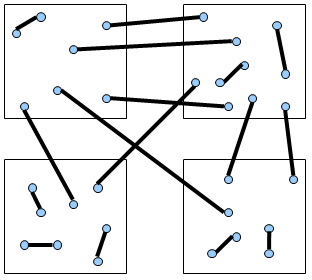
\includegraphics[width=0.5\textwidth]{cohesion_coupling_1}
		}
		\myexampletight{Low Coupling, High Cohesion}{
			\centering
			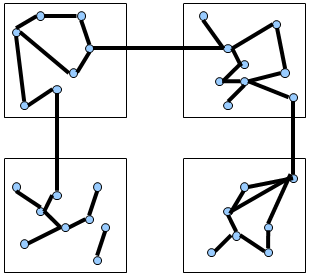
\includegraphics[width=0.5\textwidth]{cohesion_coupling_2}
		}
	\end{mycolumns}
	\begin{mycolumns}[widths={50,50},animation=none]	
	\end{mycolumns}
\end{frame}

\begin{frame}{Why Modularity?}
	\begin{mycolumns}[widths={45,55},animation=none]
		\mynote{Traditional Reasons}{			
			\begin{itemize}
				\item Modules can be developed independently of each other (collaborative work)
				\item Easier to maintain because changes can be made locally
				\item Data encapsulation promotes stability and reliability
				\item Software is easier to understand:
				\item Hiding complexity behind interfaces
				\item Modular decomposition = divide and conquer
			\end{itemize}						
		}
	\mynextcolumn
		\mynote{Modularization and Software Product Lines}{
			\begin{itemize}
				\item \emph{Reuse}: Parts of the software can be {\em reused} 
				\item \emph{Alternatives}: Modules can be {\em exchanged by alternative implementations}
				\item \emph{Variability}: Modules can be {\em reassembled in a new context} (e.g., in other projects)
			\end{itemize}
		}
		\myexampletight{}{
			\includegraphics[width=\linewidth,page=18,trim=5 115 5 5,clip]{lego} 
		}
	\end{mycolumns}	
\end{frame}

\begin{frame}{Components}
	\begin{mycolumns}[widths={50,50},animation=none]
		\mydefinition{Component \mysource{\szyperski}}{			
			A software component is a unit of composition with contractually specified \emph{interfaces} and explicit \emph{context dependencies} only. 
			A software component can be deployed independently and is \emph{subject to composition} by third parties.
		}
		\myexampletight{}{
			\centering
			\pic[width=.7\linewidth]{component_uml.png}
		}	
		\mynote{}{			
			\begin{itemize}
				\item Context/deployment dependencies: Typically container or middleware (e.g., JavaEE, COBRA, OSGi, etc.)
			\end{itemize}
		}
	\mynextcolumn
		\vspace{-0.7cm}
		\mynote{Composition and Reuse: Components}{
			\begin{itemize}
				\item Are composed with other components to form software systems,
				\item Are supposed to be re-usable in other software systems,
				\item May stem from third-party vendors (make-or-by-decisions, markets for components).
			\end{itemize}			
		}
		\myexampletight{UML Component Diagrams}{
			\centering
			\pic[width=\linewidth]{component_diagram_uml.png}
		}	
	\end{mycolumns}	
\end{frame}

\begin{frame}{Components vs. Objects/Classes}
	\begin{mycolumns}[widths={40,60},animation=none]
		\mynote{Commonalities}{			
			Lots of similar priniples, particularly 
			\begin{itemize}
				\item encapsulation and information hiding,  
				\item accessibility through public interfaces,
				\item (de-)composition and nested objects/components,
				\item etc.				
			\end{itemize}
		}
	\mynextcolumn
		\mynote{Differences}{
			\begin{itemize}
				\item \emph{Objects are smaller} than components by focusing on detailed implementation problems (components aim at abstracting from implementation details).
				\item \emph{Object are less cohesive and stronger coupled} than components due to (deliberately) delegating lots of responsibilities to other objects, while components aim at maximizing cohesion and minimizing coupling.
				\item \emph{Objects/classes are reused through inheritance and polymorphism}, while components are reused by being integrated into a component architecture.		
			\end{itemize}			
		}
	\end{mycolumns}	
\end{frame}

\begin{frame}[fragile]{Example: A Color Component}
	\begin{mycolumns}[columns=2,widths={40,60}]
			\myexample{A Reusable Component}{
				\begin{itemize}
					\item Assume that storing and printing colors is non-trivial (e.g., in our graph library). 
					\item Implement color management as a reusable component, using Java's visibility mechanism to enforce encapsulation.						
				\end{itemize}
			}
		\mynextcolumn
{\small
\begin{codetight}{}
package components.color;

~// public interface~
public class ColorComponent {
	public Color createColor(int r, int g, int b) { ~/* ... /*~ }
	public void printColor(Color color) { ~/* ... /*~ }
	public void mapColor(Object o, Color c) { ~/* ... /*~ }
	public Color getColor(Object o) { ~/* ... /*~ }
	
	~// just one component instance~
	public static ColorComponent getInstance() { return instance; }
	private static ColorComponent instance = new ColorComponent();
	private ColorComponent() { super(); }
}
public interface Color { ~/* ... /*~ }

~// hidden implementation~
class ColorImpl implements Color { ~/* ... /*~ }
class ColorPrinter { ~/* ... /*~ }
class ColorMapping { ~/* ... /*~ }
\end{codetight}
}
	\end{mycolumns}
\end{frame}

\begin{frame}[fragile]{Example: A Color Component}
	\begin{mycolumns}[columns=2,widths={60,40}]
{\small
\begin{codetight}{}
public class Graph {
	private List<Node> nodes = new ArrayList<Node>();
	public Node add() {
		Node n = null;
		@if (Config.COLORED) {
			Color c = ColorComponent.getInstance().createColor(0, 0, 0);
			n = new Node(nodes.size(), c);
		} else @ {
			n = new Node(nodes.size());
		}
		nodes.add(n);
		return n;
	}
	~// ...~
}
\end{codetight}
}
		\mynextcolumn
\vspace{-0.5cm}
{\small
\begin{codetight}{}
public class Node {
	private int id;
	@private ColorComponent colorComp =
		ColorComponent.getInstance();@
	public Node(int id) { this.id = id; }
	public Node(int id, @Color c@) {
		this(id);
		@colorComp.mapColor(this, c);@
	}
	public void print() {
		@if (Config.COLORED) {
			Color c = colorComp.getColor(this);
			colorComp.printColor(c);
		}@
		System.out.print(id);
	}
}
\end{codetight}
}			
	\end{mycolumns}
	\mynote{}{
		\begin{itemize}
			\item We can \emph{reuse} the Color Component when implementing the color feature for the graph library (but also for other applications). 
			\item However, we need to write custom code to ``connect'' our implementation with the component.\\
				$\Rightarrow$ \emph{Glue Code}
		\end{itemize}
	}
\end{frame}


\begin{frame}{Component-Based Implementation of Software Product Lines}
	\begin{mycolumns}[widths={40,60},animation=none]
		\mydefinition{General Idea}{					
			\begin{itemize}
				\item Every feature is implemented by a dedicated component.
				\item Feature selection determines which components shall be integrated to form an application.				
			\end{itemize}
		}
		\myexample{Vision}{
			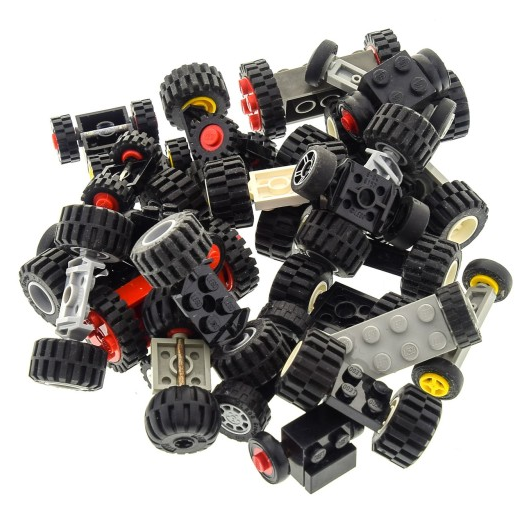
\includegraphics[width=.38\linewidth,height=1.75cm]{lego_components} 
				\vspace*{\fill}
					$\Longrightarrow$ 
				\vspace*{\fill}	
			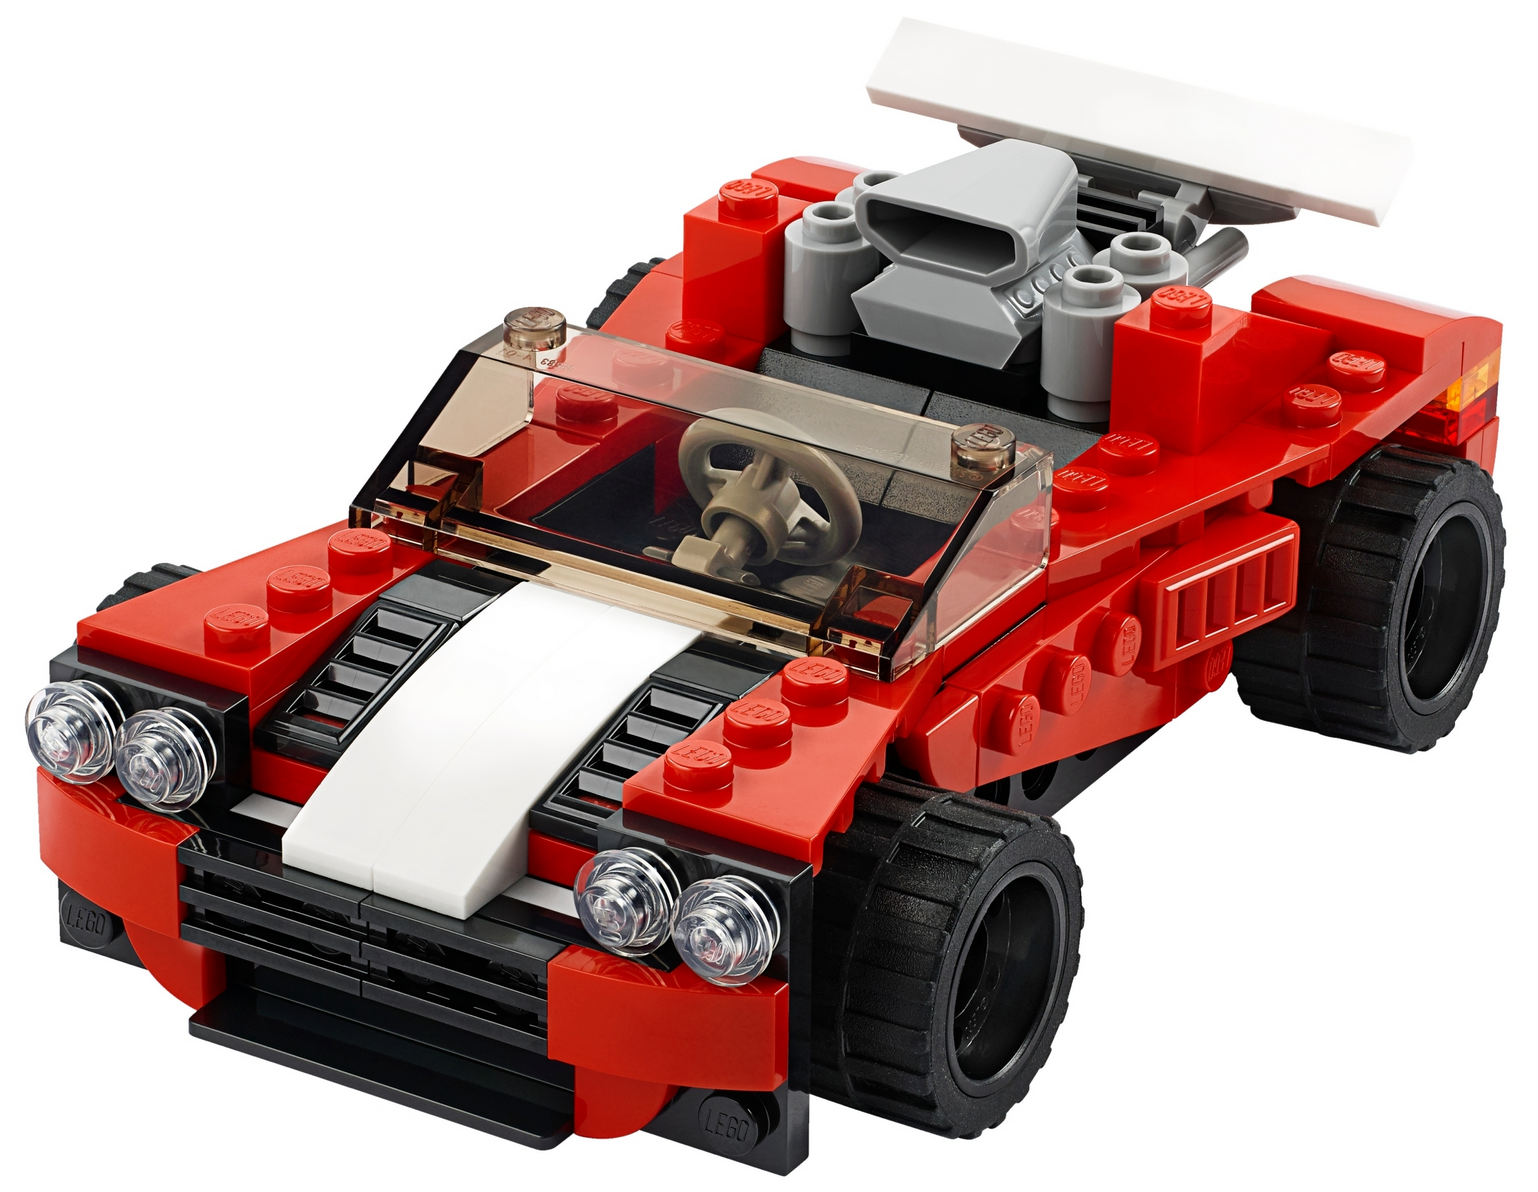
\includegraphics[width=.47\linewidth,height=1.75cm]{lego_product}
		}
	\mynextcolumn
		\myexample{Reality}{
			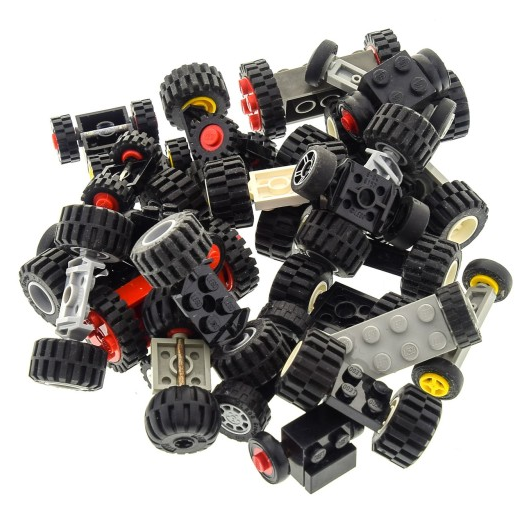
\includegraphics[width=.27\linewidth,height=1.75cm]{lego_components} 
				\vspace*{\fill}
					$+$ 
				\vspace*{\fill}	
			
\includegraphics[width=.27\linewidth,height=1.75cm]{lego_glue}
				\vspace*{\fill}
					$=$ 
				\vspace*{\fill}	
			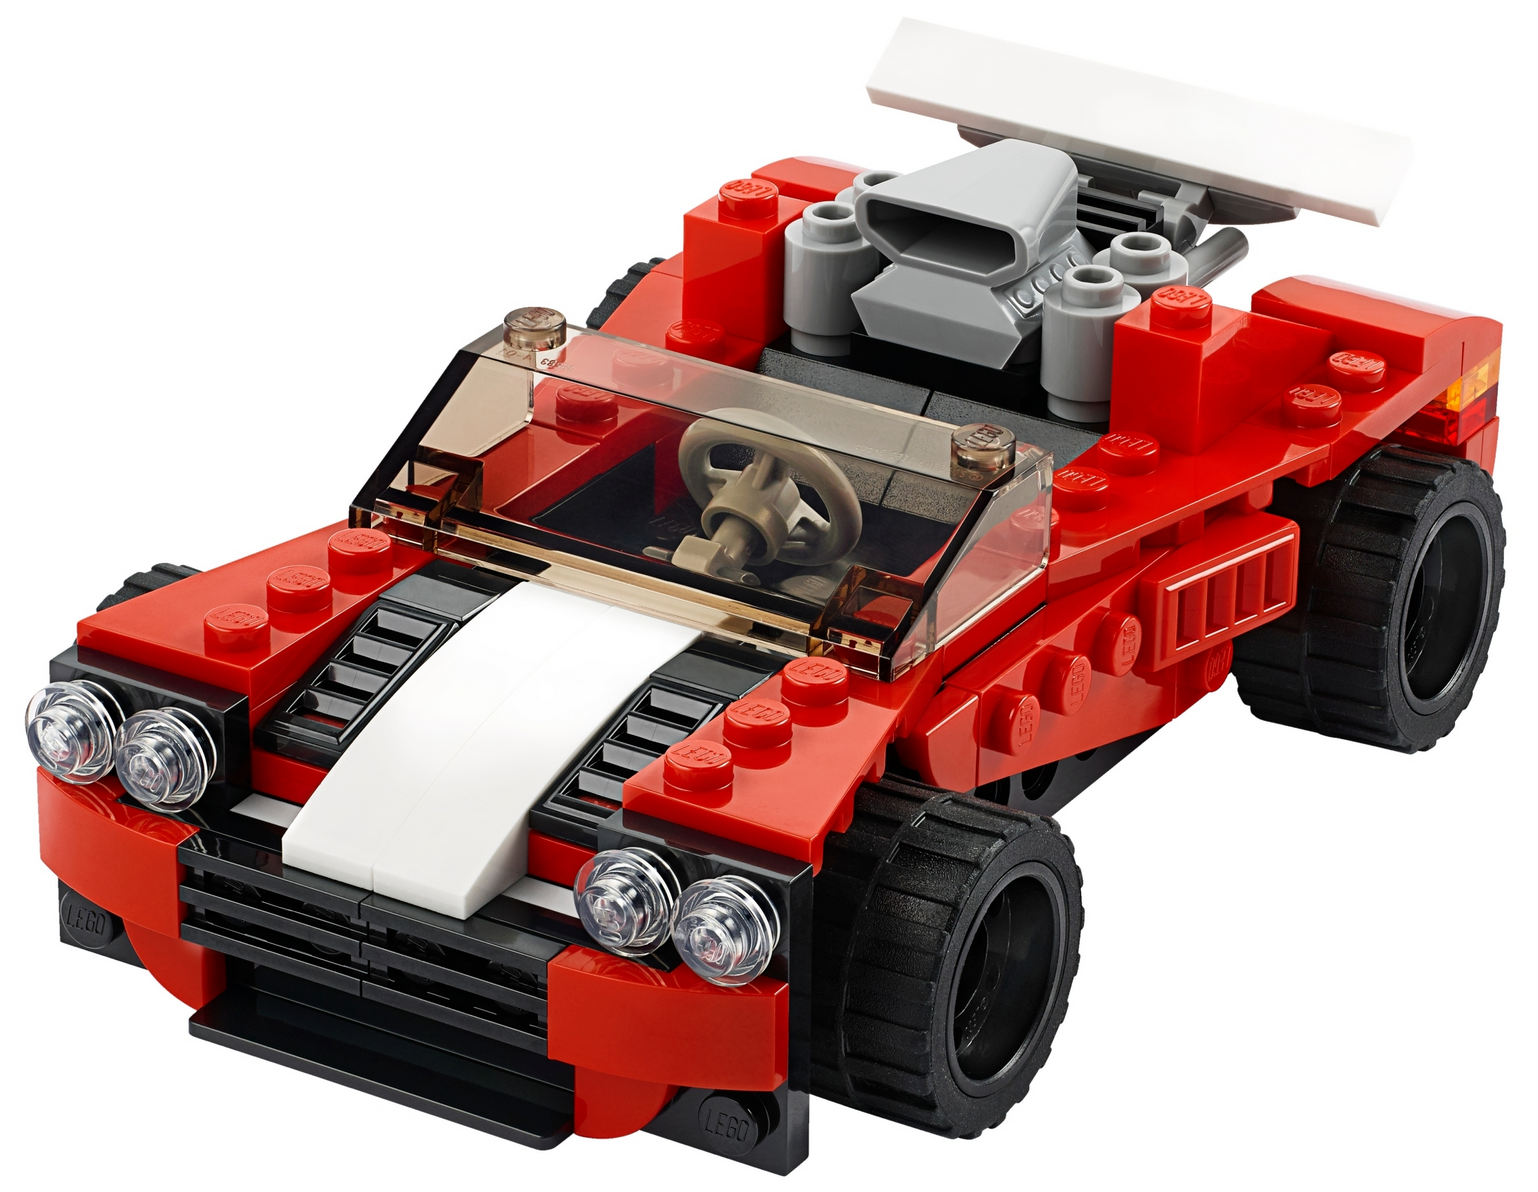
\includegraphics[width=.35\linewidth,height=1.75cm]{lego_product}
		}			
		\mynote{Glue Code and Customization}{
			\begin{itemize}
				\item Developers must connect components through glue code (exception: If components are only exchanged against alternative components)
				\item Components may contain run-time variability (e.g., color manager in our example may be parameterized by color model (RGB, CMYK, ...))
			\end{itemize}
		}
	\end{mycolumns}	
\end{frame}

\begin{frame}{The Library Scaling Problem}
TODO
\end{frame}

\subsection{Recap: UML Component Diagram}
\subsection{Vision: Component Markets}
\subsection{The Library Scaling Problem}
\subsection{Components in Java}
\subsection{Components for Features}
\subsection{Discussion}



\lessonslearned{
	\item \ldots
}{
	\item \ldots
}{
	\ldots
}

\sectionend

\section{Services and Microservices}

\subsection{(Micro-)Services}
\begin{frame}{(Micro-)Services}
	\begin{mycolumns}[widths={50,50},animation=none]
		\begin{definition}{(Micro-)Service}
			\mycite{[A (micro-)service is a module] implemented and operated as a small yet independent system, offering access to its internal logic and data through a well-defined network interface.}
				{Jamshidi et al., 2018}
		\end{definition}
		\begin{definition}{(Micro-)Service Architecture}
			\mycite{A [micro]service is a cohesive, independent process interacting via messages. 
				A microservice architecture [service-oriented architecture] is a distributed application where all its modules are microservices.}
				{Dragoni et al., 2017}
		\end{definition}
	\mynextcolumn		
		\pic[width=\linewidth]{peer-to-peer}
	\end{mycolumns}
\end{frame}

\subsection{Services vs. Components}
\begin{frame}{Services vs.\ Components}
	\begin{mycolumns}[widths={50,50},animation=none]
		\begin{definition}{Component}
			Intra-process communication (i.e., method calls)
			\begin{center}
				\pic[width=0.65\linewidth]{component_vs_service_1}
			\end{center}			
		\end{definition}
	\mynextcolumn		
		\begin{definition}{Service}
			Inter-process communication (e.g., REST API)
			\begin{center}
				\pic[width=0.65\linewidth]{component_vs_service_2}
			\end{center}	
		\end{definition}
	\end{mycolumns}
	~
	\pause
	\begin{note}{}
		As a consequence, each (micro-)service can be implemented using different technology stacks, whereas components are bound to the same technology (given by container or middleware).
	\end{note}
\end{frame}

\subsection{Microservice Architectures}
\begin{frame}{Microservice Architecture: Motivation}
	\begin{mycolumns}[widths={50,50},animation=none]
		\begin{note}{Remember: The Library Scaling Problem}
			\centering
			\pic[width=.95\linewidth]{tangram}			
		\end{note}
	\mynextcolumn		
		\pause
		\begin{note}{How small is a Microservice?}
			\begin{itemize}
				\item Components are very unspecific of how to deal with the general requirement ``not too small but not too big''.
				\item On the contrary, there is a clear philosophy behind microservice architectures, largely driven by organizational constraints wrt.\ agile teams and continuous delivery.
			\end{itemize}
		\end{note}
		\pause
		\begin{definition}{}
			\mycite{If the codebase is too big to be \emph{managed by a small team}, looking to break it down is very sensible. [...] The smaller the service, the more you \emph{maximize the benefits and downsides} of microservice architecture.}{Sam Newman, 2015}% [...] The golden rule: can you make a change to a service and deploy it by itself without changing anything else?
		\end{definition}
	\end{mycolumns}
\end{frame}

\begin{frame}{Microservice Architecture: Philosophy and Principles}
	\begin{mycolumns}[widths={50,50},animation=none]
		\begin{definition}{Conway's Law}
			\mycite{Organizations which design systems [...] are constrained to produce designs which are copies of the communication structures of these organizations.}{\href{https://www.melconway.com/Home/pdf/committees.pdf}{Melvin Edward Conway, 1968}}			
		\end{definition}
		\begin{definition}{Single Responsibility Principle}
			\mycite{Gather together the things that change for the same reasons. Separate those things that change for different reasons.}{\href{https://blog.cleancoder.com/uncle-bob/2014/05/08/SingleReponsibilityPrinciple.html}{Robert C. Martin, 2014}}			
		\end{definition}
		\begin{definition}{}
			\mycite{You build it, you run it.}{Amazon CTO Werner Vogel, 2006}			
		\end{definition}
	\mynextcolumn		
		\pause
		\begin{note}{Consequences}
			\begin{itemize}
				\item Microservices are supposed to be split along business capabilities (e.g., purchase, sale, ...) instead of technical concerns (e.g., UI, persistence, ...)
				\item Each microservice is built (full stack) {\em and} operated by a small agile team that takes over full responsibility (cf. DevOps) 
			\end{itemize}
		\end{note}
		\pause
		\begin{definition}{}
			\mycite{[A microservice] could be re-written in two weeks.}{\href{https://www.rea-group.com/blog/micro-services-what-even-are-they/}{Jon Eaves, 2014}}
		\end{definition}
		\pause
		\begin{definition}{}
			\mycite{Every team should be small enough that it can be fed with two pizzas.}{\href{https://www.theguardian.com/technology/2018/apr/24/the-two-pizza-rule-and-the-secret-of-amazons-success}{Jeff Bezos, 2018}}
		\end{definition}
	\end{mycolumns}
\end{frame}

\begin{frame}{Traditional Promises of Microservices}
	\begin{mycolumns}[widths={50,50},animation=none]
		\begin{note}{}
			\begin{itemize}
				\item \emph{Scalability}: Microservices are small enough to be developed by a small, agile team. %(cf. typical size of a Scrum team).
				\item \emph{Continuous integration/deployment}: Microservices can be deployed independently of each other. %(i.e., each microservice has its own CI/CD pipeline).
				\item \emph{Heterogeneity}: Each microservice can be implemented using its own technology stack. %(team preferences, adoption of new technologies, etc.).
				\item \emph{Fault tolerance}: The crash of a single microservice should not lead to a crash of the entire system. %(cf. design for failure).
				\item \emph{Efficiency}: Configuration of execution environment can be optimized per microservice.
				\item \emph{Modernization}: A microservice can be easily replaced by an alternative one (even re-implemented from scratch).
			\end{itemize}
		\end{note}
	\mynextcolumn
		\pause
		\begin{exampletight}{The Microservice ``Hype''}
			\pic[width=\linewidth]{microservices}

			\pause\pic[width=\linewidth]{microservices-comparison}
		\end{exampletight}
	\end{mycolumns}	
\end{frame}

\subsection{Implementation of Product Lines}
\begin{frame}{Service-Oriented Implementation of Software Product Lines}
	\begin{mycolumns}[widths={40,60},animation=none]
		\begin{example}{Recap: Component-Based Implementation}
			\pic[width=.24\linewidth,height=1.0cm]{lego_components} 
				\vspace*{\fill}
					$+$ 
				\vspace*{\fill}	
			\pic[width=.24\linewidth,height=1.0cm]{lego_glue}
				\vspace*{\fill}
					$=$ 
				\vspace*{\fill}	
			\pic[width=.3\linewidth,height=1.0cm]{lego_product}
		\end{example}	
		\begin{example}{Plenty of Glue Code}
			\centering
			\pic[width=.65\linewidth,height=2.5cm]{lego_glue}				
		\end{example}
	\mynextcolumn
		\pause
		\begin{definition}{Same Idea}
			\begin{itemize}
				\item Features are implemented as services.
				\item Feature selection determines the services to be composed.
			\end{itemize}
		\end{definition}
		\pause
		\begin{note}{However}
			``Standardized'' service composition instead of highly individual glue code.
		\end{note}
		\begin{example}{}
			\pic[width=.27\linewidth,height=1.75cm]{lego_components} 
				\vspace*{\fill}
					$+$ 
				\vspace*{\fill}	
			\pic[width=.27\linewidth,height=1.75cm]{lego_orchestration}
				\vspace*{\fill}
					$=$ 
				\vspace*{\fill}	
			\pic[width=.35\linewidth,height=1.75cm]{lego_product}
		\end{example}
	\end{mycolumns}	
\end{frame}

\subsection{Service Composition}
\begin{frame}{\myframetitle}
	\begin{mycolumns}[t]
		\begin{definition}{Orchestration \deutsch{Orchestrierung}}
			Description of an executable (business-)process as a combination of services (centralized perspective).
		\end{definition}
		\begin{example}{}
			\href{https://docs.oasis-open.org/wsbpel/2.0/wsbpel-v2.0.html}{Web Services Business Process Execution Language (WS-BPEL)}
		\end{example}

		\centering\pic[height=35mm]{trafficlights}
	\mynextcolumn
		\begin{definition}{Choreography \deutsch{Choreographie}}
			Each service describes its own task within a service composition (decentralized perspective).
		\end{definition}
		\begin{example}{}
			\href{https://www.w3.org/TR/ws-cdl-10/}{Web Services Choreography Description Language (WS-CDL)}
		\end{example}

		\centering\pic[height=35mm]{crossroad}
	\end{mycolumns}	
\end{frame}

\lessonslearned{
	\item \ldots
}{
	\item \ldots
}{
	\ldots
}

\sectionend

\section{Black-Box Frameworks}

% TODO this whole part is inconsistent with the naming of extension points / hot spots. would recommend to only use extension point and just mention hot spot once.

\subsection{Hot Spots and Plug-Ins}
\begin{frame}{Framework with Plug-Ins}
	\begin{fancycolumns}[b]
		\begin{definition}{Framework and Hot Spot \mysource{\fospl\mypages{80--81}}}
			A \emph{framework} is a set of classes that embodies an abstract design for solutions to a family of related problems, and supports reuse at a larger granularity than classes. A framework is open for \emph{extension} at explicit \emph{hot spots} (aka.\ extention point).
		\end{definition}
		\begin{definition}{Plug-In \mysource{\fospl\mypages{80--81}}}
			A \emph{plug-in} extends hot spots of a [...] framework with custom behavior. A plug-in can be separately compiled and deployed.	
		\end{definition}
		\begin{note}{}
			Frameworks with plug-ins are also called \emph{black-box frameworks}: Developers need to understand interfaces, but not the internal framework implementation.
		\end{note}
	\nextcolumn
		\vspace{-12mm}
		\begin{note}{Inversion of Control}
			Hollywood principle: \mycite{Don't call us, we call you}

			\centering 
			\picDark[width=0.8\linewidth]{library_vs_framework}
		\end{note}
		\begin{note}{}
			\begin{itemize}
				\item Can be understood in terms of the observer and/or strategy pattern: The framework exposes explicit hot spots, at which plug-ins can register observers and strategies.
				\item Requires \emph{preplanning} for possible future extensions
			\end{itemize}
		\end{note}
	\end{fancycolumns}
\end{frame}

\subsection{Preplanned Extensions}
\begin{frame}{Real-World Example: Preplanned Bike Extensions}
	\begin{fancycolumns}[columns=4,T]
		\centering\pic[width=\linewidth]{bike-extensionpoint1}

		bike lock
	\nextcolumn
		\centering\pic[width=\linewidth]{bike-extensionpoint2}

		front wheel brake
	\nextcolumn
		\centering\pic[width=\linewidth]{bike-extensionpoint3}

		rear wheel brake
	\nextcolumn
		\centering\pic[width=\linewidth]{bike-extensionpoint4}

		kickstand
	\end{fancycolumns}
\end{frame}

\begin{frame}{Real-World Example: Preplanned Bike Extensions}
	\begin{fancycolumns}[columns=5,widths={30,5,30,5,30}]
		\centering\pic[width=\linewidth]{bike-extensionpoint1-withoutplugin}

		framework with extension~points
	\nextcolumn
		\centering\Huge +
	\nextcolumn
		\centering\pic[width=\linewidth]{bike-lock}

		plug-ins\\~
	\nextcolumn
		\centering\Huge =
	\nextcolumn
		\centering\pic[width=\linewidth]{bike-extensionpoint1}

		framework with plug-ins\\~
	\end{fancycolumns}
\end{frame}

\subsection{Basic Design Principles}
\begin{frame}{Simple Java Example: A Family of Dialogs \mytitlesource{\fospl}}
	\begin{fancycolumns}
		\begin{exampletight}{}
			\centering \pic[width=0.8\linewidth]{dialog1}
		\end{exampletight}
		\begin{exampletight}{}
			\centering \pic[width=0.8\linewidth]{dialog2}
		\end{exampletight}
		\begin{exampletight}{}
			\centering \pic[width=\linewidth]{dialog3}
		\end{exampletight}
	\nextcolumn		
		\begin{note}{}
			\begin{itemize}
				\item All dialogs have a similar structure (basically textfield + button)
				\item Large parts of the source code are identical:
				\begin{itemize}
					\item Main method,
					\item Initialization of windows, textfield and button
					\item layouting,
					\item window closing and disposal,
					\item etc.
				\end{itemize}
			\end{itemize}
		\end{note}	
	\end{fancycolumns}
\end{frame}
	
\begin{frame}[fragile]{Simple Java Example: A Family of Dialogs}
	\vspace{-2mm}
	\begin{fancycolumns}[b]
\begin{codetight}{}
public class Calc extends JFrame {
	private JTextField textfield;
	public static void main(String[] args) {
		new Calc().setVisible(true);
	}
	public Calc() { init(); }
	protected void init() {
		JPanel p = new JPanel(new BorderLayout());
		p.setBorder(new BevelBorder(/* ... */));
		JButton button = new JButton();
		button.setText(@"calculate"@);
		p.add(button, BorderLayout.EAST);
		textfield = new JTextField("");
		textfield.setText(@"10 / 2 + 6"@);
		textfield.setPreferredSize(new Dimension(350, 40));
		p.add(textfield, BorderLayout.WEST);
		button.addActionListener(new ActionListener() 
			{ @/* calculate */@ });
		this.setContentPane(p);
		this.setTitle(@"My Great Calculator"@);
		this.pack();
		// ...
	}
}
\end{codetight}
		\nextcolumn
\begin{codetight}{}
public class Ping extends JFrame {
	private JTextField textfield;
	public static void main(String[] args) {
		new Calc().setVisible(true);
	}
	public Calc() { init(); }
	protected void init() {
		JPanel p = new JPanel(new BorderLayout());
		p.setBorder(new BevelBorder(/* ... */));
		JButton button = new JButton();
		button.setText(@"ping"@);
		p.add(button, BorderLayout.EAST);
		textfield = new JTextField("");
		textfield.setText(@"127.0.0.1"@);
		textfield.setPreferredSize(new Dimension(350, 40));
		p.add(textfield, BorderLayout.WEST);
		button.addActionListener(new ActionListener() 
			{ @/* calculate */@ });
		this.setContentPane(p);
		this.setTitle(@"Ping"@);
		this.pack();	
		// ...
	}
}
\end{codetight}
	\end{fancycolumns}
\end{frame}


\begin{frame}[fragile]{Simple Java Example: A Family of Dialogs}
	\vspace{-2mm}
	\begin{fancycolumns}
		\begin{note}{}
			plug-in implementation hidden from application
		\end{note}
\begin{codetight}[basicstyle=\tiny]{}
public class Application extends JFrame {
	private Plugin plugin;
	// ...
	public Application(@Plugin plugin@) {
		@this.plugin = plugin;
		plugin.setApplication(this);@
		init();
	}
	protected void init() {
		JPanel p = new JPanel(new BorderLayout());
		p.setBorder(new BevelBorder(/*...*/);
		JButton button = new JButton();
		button.setText(@plugin.getButtonText()@);
		p.add(button, BorderLayout.EAST);
		textfield = new JTextField("");
		textfield.setText(@plugin.getInitialText()@);
		textfield.setPreferredSize(new Dimension(200, 20));
		p.add(textfield, BorderLayout.WEST);		
		button.addActionListener(/*... @plugin.buttonClicked();@ ...*/);
		this.setContentPane(p);		
		this.setTitle(@plugin.getApplicationTitle()@);
		// ...
	}
	@public String getInput() {
		return textfield.getText();
	}@
}
\end{codetight}
		\nextcolumn
{
\begin{codetight}[basicstyle=\tiny]{}
public interface Plugin {
	String getApplicationTitle();
	String getButtonText();
	String getInitialText();
	void buttonClicked();
	void setApplication(Application app);
}
\end{codetight}
\begin{codetight}[basicstyle=\tiny]{}
public class CalcPlugin implements Plugin {
	private Application application;

	public String getApplicationTitle() {
		return "My Great Calculator";
	}
	public String getButtonText() {
		return "calculate";
	}
	public String getInitialText() {
		return "10 / 2 + 6";
	}
	public void buttonClicked() {
		calculate(application.getInput());
	}
	public void setApplication(Application app) {
		application = app;
	}
	private void calculate(String expression) {
		/* calculate */
	}
}
\end{codetight}
}
	\end{fancycolumns}
\end{frame}

\begin{frame}[fragile]{Simple Example: A Family of Dialogs}
	\begin{fancycolumns}
		\begin{note}{}
			application implementation hidden from plug-in
		\end{note}
\begin{codetight}[basicstyle=\tiny]{}
public class Application extends JFrame @implements InputProvider@ {
	private Plugin plugin;
	// ...
	public Application(Plugin plugin) {
		this.plugin = plugin;
		@plugin.setInputProvider(this);@
		init();
	}
	protected void init() {
		JPanel p = new JPanel(new BorderLayout());
		p.setBorder(new BevelBorder(/*...*/);
		JButton button = new JButton();
		button.setText(plugin.getButtonText());
		p.add(button, BorderLayout.EAST);
		textfield = new JTextField("");
		textfield.setText(plugin.getInitialText());
		textfield.setPreferredSize(new Dimension(200, 20));
		p.add(textfield, BorderLayout.WEST);		
		button.addActionListener(/* . . . plugin.buttonClicked(); . . . */);		
		// ...
	}
	public String getInput() {
		return textfield.getText();
	}
}
\end{codetight}
		\nextcolumn
{
\begin{codetight}[basicstyle=\tiny]{}
public interface InputProvider {
	public String getInput();
}
\end{codetight}
\begin{codetight}[basicstyle=\tiny]{}
public interface Plugin {
	String getApplicationTitle();
	String getButtonText();
	String getInitialText();
	void buttonClicked();
	@void setInputProvider(InputProvider p);@
}
\end{codetight}
\begin{codetight}[basicstyle=\tiny]{}
public class CalcPlugin implements Plugin {
	@private InputProvider inputProvider;@

	public String getApplicationTitle() { /*...*/ }
	public String getButtonText() { /*...*/ }
	public String getInitialText() { /*...*/ }
	public void buttonClicked() {
		calculate(@inputProvider.getInput()@);
	}
	@public void setInputProvider(InputProvider p) {
		inputProvider = p;
	}@
	private void calculate(String expression) {
		/* calculate */
	}
}
\end{codetight}
}
	\end{fancycolumns}
\end{frame}

\subsection{Plug-In Loading and Management}
\begin{frame}{Plug-In Loading and Management}
	\begin{fancycolumns}
		\begin{note}{Simple Example vs.\ Reality}
			simplification in our previous example:
			\begin{itemize}
				\item a single extension point supporting the registration of a single plug-in 
				\item plug-in implementation known at compile-time 
			\end{itemize}
			typical requirements in practice:
			\begin{itemize}
				\item an extension point typically supports the registration of arbitrarily many plug-ins
				\item a single plug-in may extend several extension points
				\item a plug-in may add new extension points to the framework (framework of frameworks)
				\item plug-in implementation provided by third parties %(requires load-time variability) % TODO sounds wrong to me (Thomas)
			\end{itemize}
		\end{note}
	\nextcolumn
		\begin{definition}{Plug-In Loader}
			\begin{itemize}
				\item Searches in a dedicated directory for DLL/JAR/XML files
				\item Tests whether file implements a plug-in
				\item Checks dependencies
				\item Initializes plug-ins
			\end{itemize}
		\end{definition}
		\begin{definition}{Plug-In Manager}
			GUI and/or console interface for plug-in administration and configuration
		\end{definition}
	\end{fancycolumns}
\end{frame}

\begin{frame}[fragile]{Example: Plug-In Loading and Management}
	\begin{fancycolumns}[t]
\begin{codetight}{Plug-In Loader using Java Reflection}
public class Starter {
	public static void main(String[] args) {
		if (args.length != 1)
			System.out.println("Plugin name not specified");
		else {
			String pluginName = args[0];
			try {
				Class pluginClass = Class.forName(pluginName);
				new Application((Plugin) 
					pluginClass.newInstance()).setVisible(true);
			} catch (Exception e) {
				System.out.println("Cannot load plugin " + 
					pluginName + ", reason: " + e);
			}
		}
	}
}
\end{codetight}
		\nextcolumn
\begin{codetight}{Handling multiple Plug-Ins}
public class Application {
	private List<Plugin> plugins;

	public Application(List<Plugin> plugins) {
		this.plugins = plugins;
		for (Plugin plugin : plugins) {
			plugin.init();
		}
	}

	public Message processMsg(Message msg) {
		for (Plugin plugin : plugins) {
			msg = plugin.process(msg);
			// ...
		}
		return msg;
	}
}
\end{codetight}
	\end{fancycolumns}
\end{frame}

\subsection{Frameworks in the Wild}
\begin{frame}{Frameworks in the Wild: Eclipse}
	\begin{fancycolumns}[widths={70},animation=none]
		\pic[width=\linewidth]{eclipse_overview}
	\nextcolumn
		\vspace{-0.7cm}
		\begin{example}{Versatile IDE}
			\begin{itemize}
				\item Lots of common functionality required by any IDE
					(e.g., editors, incremental project build, etc.) 
				\item Only language-specific extensions need to be registered
					(e.g., syntax highlighting, compiler, etc.)
			\end{itemize}
		\end{example}
		\pause
		\begin{note}{Specifically in Eclipse}
			\begin{itemize}
				\item Actually a set of (recursively nested) frameworks
				\item Largely declarative description of extension points
			\end{itemize}
		\end{note}
	\end{fancycolumns}
\end{frame}

\begin{frame}{Frameworks in the Wild: Eclipse \mytitlesource{\featureide}}
	\begin{fancycolumns}%[forget]
		\pic[width=\linewidth]{framework-with-plugins}
	\nextcolumn
		\pic[width=\linewidth]{framework-a-plugin}
	\end{fancycolumns}
\end{frame}

\begin{frame}{Frameworks in the Wild: Further Examples}
	\begin{fancycolumns}[columns=3,widths={15,70},animation=none]
	\nextcolumn
		\begin{example}{}
			\begin{itemize}
				\item Other IDEs (e.g., IntelliJ)
				\item Unit test frameworks (e.g., JUnit)
				\item Frontend frameworks (e.g., React, Angular)
				\item Backend frameworks (e.g., Spring Boot, Ruby on Rails, Django) 
				\item Multimedia frameworks (e.g., DirectX)
				\item Raster/vector graphics editors (e.g., Adobe Photoshop, MS Visio)
				\item Instant messenger frameworks (e.g., Miranda, Trillian)
				\item Compiler frameworks (e.g., LLVM, Polyglot, abc, JustAddJ)
				\item Web browsers (e.g., Firefox)
				\item E-Mail clients (e.g., Thunderbird)
				\item etc.
			\end{itemize}
		\end{example}		
	\nextcolumn
	\end{fancycolumns}
\end{frame}

\subsection{Implementation of Product Lines}
\begin{frame}<1-4>[label=SPLwithPlugIns]
	\frametitle<1-4>{Framework-Based Implementation of Software Product Lines}
	\frametitle<5>{\myframetitle}
	\begin{fancycolumns}[widths={40},animation=none]
		\begin{example}{Recap: Service-Based Implementation}
			\raisebox{-0.4cm}{\pic[width=.23\linewidth,height=1.0cm]{lego_components}}
			$+$ 
			\raisebox{-0.4cm}{\pic[width=.23\linewidth,height=1.0cm]{lego_orchestration}}
			$=$
			\raisebox{-0.4cm}{\pic[width=.3\linewidth,height=1.0cm]{lego_product}}
		\end{example}
		\begin{example}{Still needs some specification of ``composition'' (cf.\ orchestration vs.\ choreography)}
			\centering
			\pic[width=.65\linewidth,height=2.5cm]{lego_orchestration}				
		\end{example}
	\nextcolumn		
		\pause
		\begin{definition}{Same Idea}
			\begin{itemize}
				\item Features are implemented by different plug-ins
				\item Feature selection determines the plug-ins to be loaded and registered 
			\end{itemize}
		\end{definition}
		\pause
		\begin{note}{}
				neither glue code nor explicit service composition required
		\end{note}
		\begin{example}{}
			\raisebox{-0.8cm}{\pic[width=.29\linewidth,height=1.75cm]{lego_product_partial}}
			$+$
			\raisebox{-0.8cm}{\pic[width=.27\linewidth,height=1.75cm]{lego_components}}
			$=$
			\raisebox{-0.8cm}{\pic[width=.29\linewidth,height=1.75cm]{lego_product}}
		\end{example}
		\pause
		\begin{note}{}
				full automation comes at a price (cf.\ preplanning problem)
		\end{note}		
	\end{fancycolumns}	
\end{frame}

\begin{frame}[fragile,label=GraphsWithPlugins]{Example: Extending Basic Graphs by Plug-Ins?}
	\begin{fancycolumns}
\begin{codetight}[basicstyle=\tiny]{}
public class Graph {
	@private List<GraphPlugin> plugins = new ArrayList<GraphPlugin>();@
	// ...	
	@public void registerPlugin(GraphPlugin p){
		plugins.add(p);
	}@
	public void addNode(int id, Color c){
		Node n = new Node(id);
		@notifyAdd(n, c);@
		nodes.add(n);
	}
	public void print() {
		for (Node n : nodes) {
			@notifyPrint(n);@
			// ...
		}
		// ...
	}
	@private void notifyAdd(Node n, Color c) {
		for (GraphPlugin p : plugins) {
			p.aboutToAdd(n, c);
		}
	}
	private void notifyPrint(Node n) {
		for (GraphPlugin p : plugins) {
			p.aboutToPrint(n);
		}
	}@
	// ...
}
\end{codetight}
		\nextcolumn
\begin{codetight}[basicstyle=\tiny]{}
public interface GraphPlugin {
	public void aboutToAdd(Node n, Color c);
	public void aboutToAdd(Edge e, Weight w);
	public void aboutToPrint(Node n);
	public void aboutToPrint(Edge e);
}
\end{codetight}
\begin{codetight}[basicstyle=\tiny]{}
public class ColorPlugin implements GraphPlugin {
	private Map<Node, Color> map = new HashMap<Node, Color>();

	public void aboutToAdd(Node n, Color c) {
		map.put(n, c);
	}
	
	public void aboutToAdd(Edge e, Weight w) {
		~// do nothing~
	}
	
	public void aboutToPrint(Node n) {
		Color c = map.get(n);
		Color.setDisplayColor(c);
	}
	
	public void aboutToPrint(Edge e) {
		~// do nothing~
	}
}
\end{codetight}
	\end{fancycolumns}
\end{frame}

\subsection{Discussion}
\begin{frame}<1-2>[label=ChallengesOfPlugins]
	\frametitle<1-2>{Challenges and Problems}
	\frametitle<3>{\myframetitle}
	\begin{fancycolumns}
		\begin{example}{}
			In our example, we can observe that:
			\begin{itemize}
				\item There are lots of empty methods in the ColorPlugin 
				\item The Framework consults all registered plug-ins before printing a node or edge
			\end{itemize}
		\end{example}		
		\begin{definition}{General Challenge: Cross-cutting Concerns}
			Implementing cross-cutting concerns as plug-ins 
			\begin{itemize}				
				\item typically leads to huge interfaces, large parts of which are irrelevant for a dedicated plug-in 
				\item causes lots of communication overhead between plug-ins and framework
			\end{itemize}
		\end{definition}
	\nextcolumn
		\begin{example}{}
			If we were not familiar with our graph library, would we anticipate that:
			\begin{itemize}
				\item Colors and weights should be part of the Plugin interface?
				\item Every plug-in needs to be notified that the framework is about to print a node or edge? 
			\end{itemize}
		\end{example}
		\begin{definition}{Generally known as Preplanning Problem}
			\begin{itemize}
				\item Hard to identify and foresee the relevant hot spots and nature of extensions
				\item Developing a framework needs lots of expertise and excellent domain knowledge 
			\end{itemize}
		\end{definition}
	\end{fancycolumns}
\end{frame}


\lessonslearned{
	\item \ldots
}{
	\item \ldots
}{
	\ldots
}

\mode<beamer>{
	\begin{frame}{\inserttitle}
		\lectureseriesoverview
	\end{frame}

	\contentoverview
}


\end{document}
